\chapter{Einf\"uhrung}
\label{chap:introduction}
Tagt{\"a}glich tauschen Millionen von Nutzern {\"u}ber Social Media Informationen zu verschiedenen Themen aus. Eine der bekanntesten Plattformen ist Twitter: eine Microblogging-Plattform, die sich grosser Beliebtheit erfreut und weltweit eingesetzt wird. Microblogging ist eine spezielle Form des Bloggens und unterscheidet sich vom klassischen Blogging vor allem durch die L{\"a}nge der Eintr{\"a}ge. Seit November 2017 betr{\"a}gt die maximale L{\"a}nge der Nachrichten auf Twitter 280 Unicode-Zeichen. Standardm{\"a}ssig ist ein Beitrag, ein sogenannter ``Tweet'', {\"o}ffentlich und auch f{\"u}r nicht registrierte Benutzer sichtbar. Die Tweets werden haupts{\"a}chlich den Followern angezeigt, aber {\"u}ber Hashtags und/oder Links oder Retweets kann eine breite Masse auf der ganzen Welt erreicht werden.

Leider haben Hasskommentare, Trolling und Social Media Mobbing in den letzten Jahren zugenommen und sind zu einem ernsthaften Problem geworden. Daf{\"u}r gibt es unterschiedliche Gr{\"u}nde, die zu diesem Anstieg f{\"u}hren: Ein Grund ist sicher die Anonymit{\"a}t des Internets, denn es ist leichter einen abf{\"a}lligen Kommentar zu schreiben, als ihn der betreffenden Person direkt ins Gesicht zu sagen. Doch dies ist nicht die einzige Erkl{\"a}rung. Generell ist zu beobachten, dass sich vermehrt Prominente wie Donald Trump, Jens Maier und Thomas Seitz - letztere beide aus der AfD - oder Josh Hader (Baseballspieler), um nur einige wenige zu nennen, rassistisch in Social Media Kan{\"a}len {\"a}ussern. Durch diesen t{\"a}glichen Gebrauch und der Verbreitung von Hasskommentaren durch Prominente scheint die {\"o}ffentliche Diskreditierung in der Gesellschaft f{\"u}r viele akzeptabel geworden zu sein. 

Doch was genau sind Hasskomentare? Hier eine englische Definition: 
\begin{description}
\item[hate speech] speech that attacks, threatens, or insults a person or group on the basis of national origin, ethnicity, color, religion, gender, gender identity, sexual orientation, or disability.  \url{https://www.dictionary.com/browse/hate-speech}
\end{description}

Beispiele f{\"u}r rassistische oder sexistische Tweets sind:
\begin{itemize}
  \item $@$thumpmomma: I likewise saw militant Muslims burning our flag and burning George Bush photos and figures, right after 9/11! Not\#here!
  \item $@$femfreq the main reason why all the harass to women is because of all the dumb feminist bitches who want to be superior. Hope u die raped
  \item Sir\_Penaut 1.You din't go to colleg. 2. You are black.
  \item You're studying Computer Science? Do you wanna meet boys there and change university when you tried them all?" \#EverydaySexism
  \item Experience Charlie. Married woman who loves hot phone sex with strangers. Can you get me off? - 27 http://t.co/bpDqqPoGAe
\end{itemize}
                                                                                                                                                                                                                                                                                                                                                                                                                                                                                                                                                                                                                                                                                                                                                                                                                                                                                                                                                                                                                                                                                                                                                                                                                                                                                                                                                                                                                                                                                                                                                                                                                                                                                                                                                                                                                                                                                                                                                                       
Die oben aufgef{\"u}hrten Tweets sind in Englisch, da die Modelle (siehe Kapitel \ref{sec:introduction_purpose}) mit englischen Trainingsdaten trainiert wurden und die im CAS Practical Machine Learning (PML) entwickelte, hier weiter verwendete App nur englischen Text klassifizieren kann.                                                                                                                                                                                                                                                                                                                                                                                                                                                                                                                                                                                                                                                                                                                                                                                                                                                                                                                                                                                                                                                                                                                                                                                                                                                                                                                                                                                                                                                                                                                                                                                                                                                                                                                                                                                                                                                                                                                                                                                                                                                                                                                                                                                                                                                                                                                                                                                                                                                                                                                                                                                                                                                                                                                                                                                                                                                                                                                                                                                                                                                                                                                                                                                                                                                                                                                                                                                                                                                                                                                                                                                                                                                                                                                                                                                                                                                                                                                                                                                                                                               

\begin{figure}[H]
	\centering
		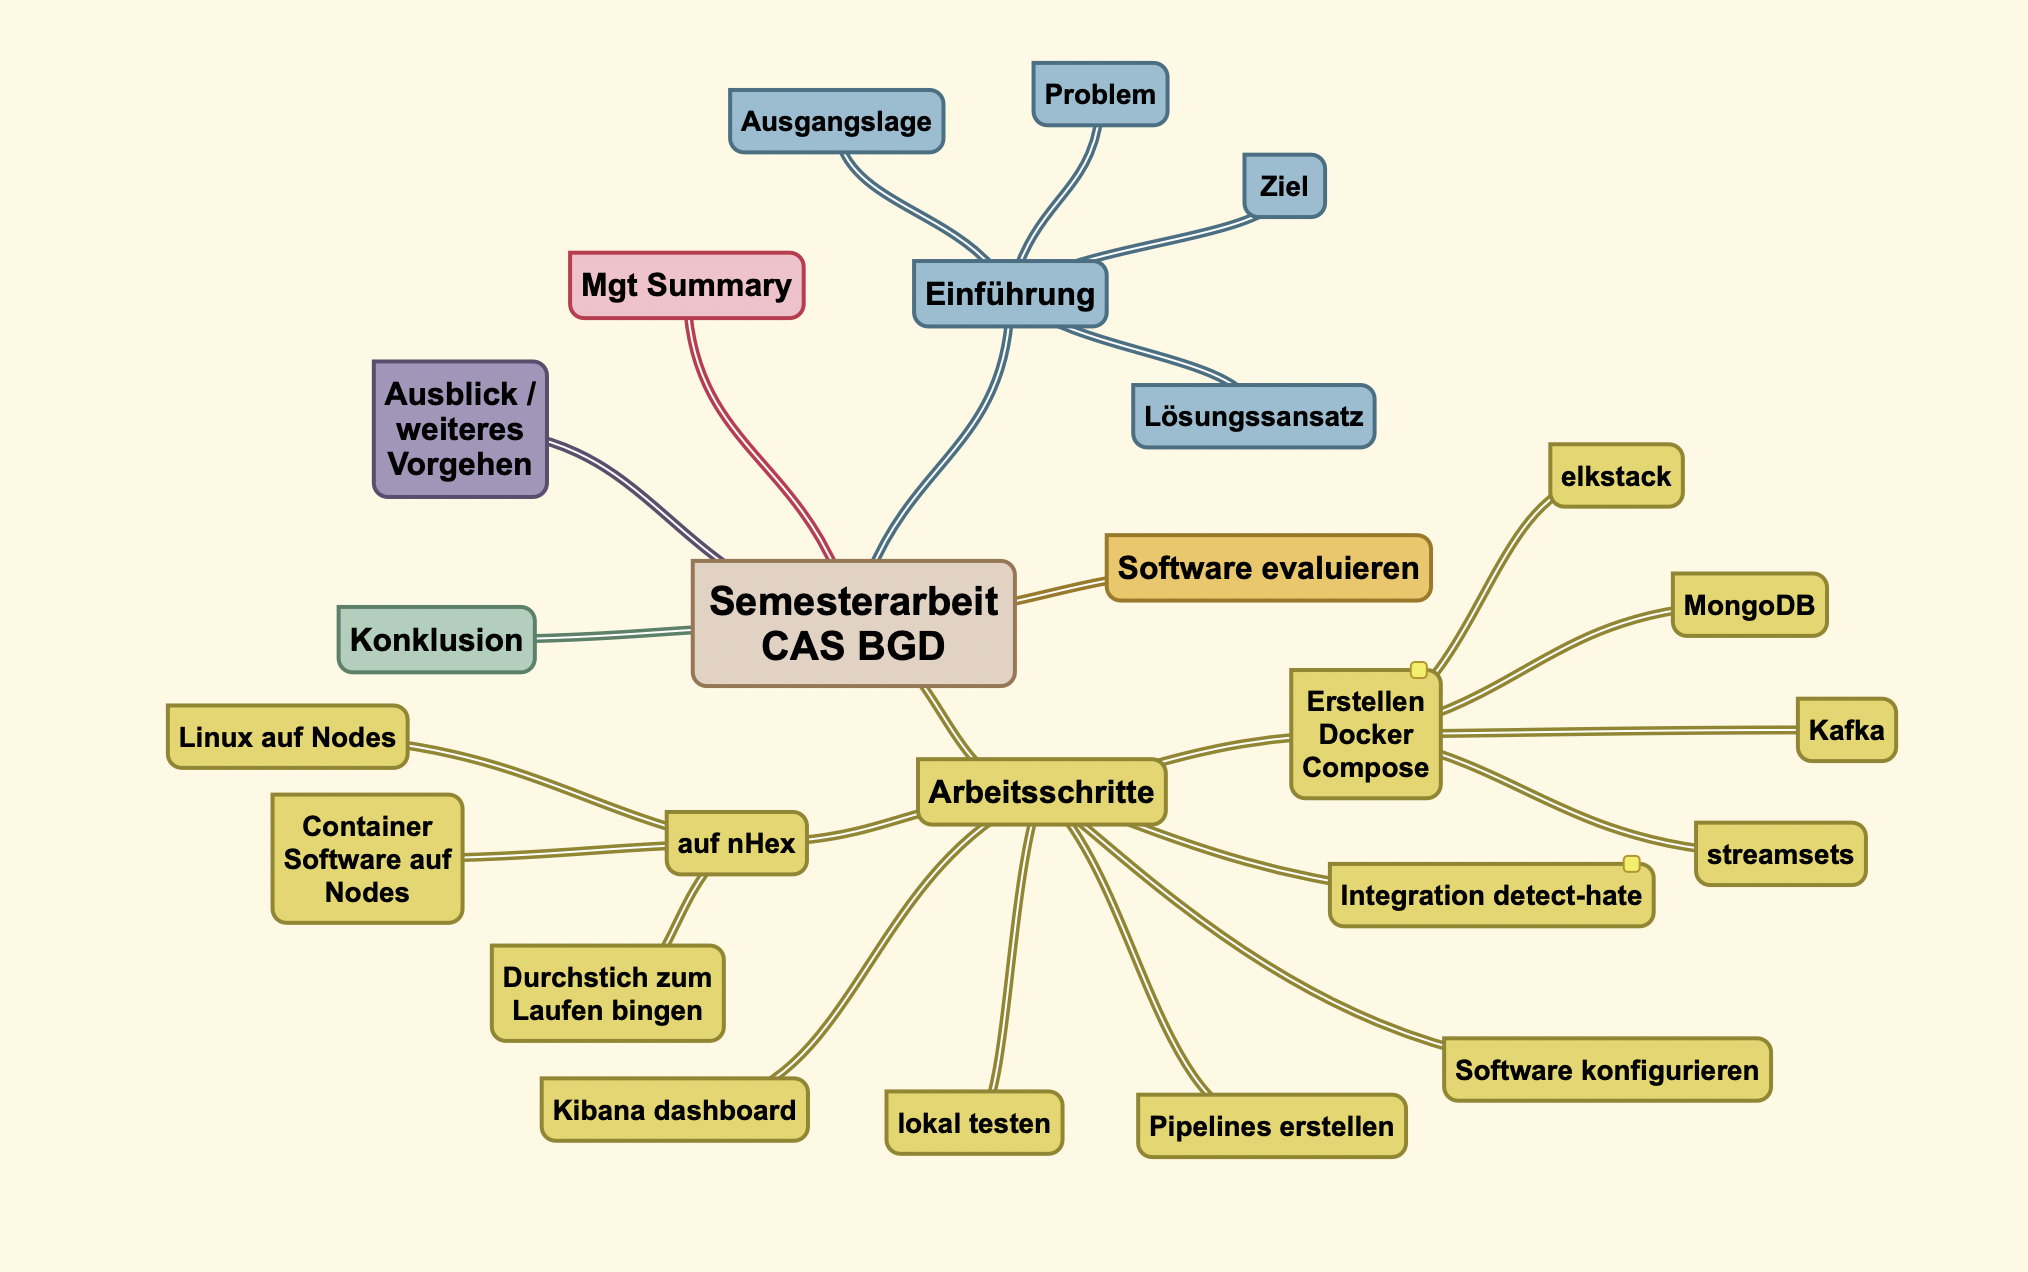
\includegraphics[scale=0.4 ]{images/inhalt_arbeit.png}
	\caption{Inhalt Semsterarbeit}
	\label{fig:inhalt_semesterarbeit}
\end{figure}

Das Mindmap zum Vorgehen und Aufbau dieser Semesterarbeit ist in Abbildung \ref{fig:inhalt_semesterarbeit} dargestellt. Die hier folgende Dokumentation orientiert sich an der dargestellten Struktur. 

                                                                                                                                                                                                                                                                                                                                                                                                                                                                                                                                                                                                                                                                                                                                                                                                                                                                                                                                                                                                                                                                                                                                                                                                                                                                                                                                                                                                                                                                                                                                                                                                                                                                                                                                                                                                                                                                                                                                                                                                                                                                                                                                                                                                                                                                                                                                                                                                                                                                                                                                                                                                                                                                                                                                                                                                                                                                                                                                                                                                                                                                                                                                                                                                                                                                                                                                                                                                                                                                                                                                                                                                                                                                                                                                                                                                                              \section{Ausgangslage}
\label{sec:introduction_purpose}

Im CAS Practical Machine Learning wurde eine \href{http://www.detect-hate.com}{Python Flask App} entwickelt um Hasskommentare (hate speech) in Tweets zu erkennen. F{\"u}r die Klassifikation wurden folgende Algorithmen verwendet und 20 Modelle trainiert:
\begin{itemize}
\item Lineare Support Vector Machine (SVM)
\item Logistic Regression
\item Multinominal Naive Bayes
\item Long short-term memory (LSTM) neuronales Netz
\end{itemize}
Die Anzahl der Modelle ergibt sich aus der Zweischrittklassifikation. Zuerst wird ermittelt ob ein Tweet Hasskommentare enth{\"a}lt. Falls dies der Fall ist wird ermittelt ob der Tweets rassistische oder sexistische Inhalte hat. Da es vier Algorithmen sind, die verwendet wurden und bei jedem zweiten Klassifikator zus{\"a}tzlich je ein Modell f{\"u}r up- und down sampling trainiert worden ist, ergeben sich in Summe 20 verschiedene, einzeln trainierte Modelle:

\begin{itemize}
  \item 4 Modelle f{\"u}r den ersten Klassifikationsschritt
  \item 4 Modelle f{\"u}r rassistische Tweets mit up sampling
  \item 4 Modelle f{\"u}r rassistische Tweets mit down sampling
  \item 4 Modelle f{\"u}r sexistische Tweets mit up sampling
  \item 4 Modelle f{\"u}r sexistische Tweets mit down sampling
\end{itemize}

Ein up resp. down sampling wurde gemacht um die Performance sowie die Qualit{\"a}t der Modelle vergleichen zu k{\"o}nnen.

Als Datengrundlage f{\"u}r die Modelle dienten vier unterschiedliche Datens{\"a}tze aus verschiedenen Quellen mit total ca. 85'000 Tweets. Diese Datens{\"a}tze enthielten nebst den eigentlichen Tweets weitere Spalten, so z.B. die folgenden Labels:
\begin{itemize}
  \item None
  \item Abusive
  \item Sexist
  \item Racist
\end{itemize}
Basierend auf den verwendeten Datens{\"a}tzen und deren Labels wurden die oben genannten Klassifikationsalgorithmen und das Neuronale Netz trainiert, um auch neue, den Modellen bis dato unbekannte Tweets klassifizieren zu k{\"o}nnen. 

\section{Problemstellung }
\label{sec:introduction_	purpose}
Es war noch nicht m{\"o}glich die Tweets mit der App aus dem CAS PML automatisch, direkt ab Twitter zu klassifizieren. Um zu pr{\"u}fen ob ein Text Hasskommentare enth{\"a}lt ist ein manueller Zwischenschritt n{\"o}tig, bei welchem die Tweets von Twitter kopiert und auf der Webseite \href{http://www.detect-hate.com}{www.detect-hate.com} in das Textfeld eingef{\"u}gt wird. Das Resultat, also die Klassifikation ob der Tweet Hasskommentare enth{\"a}lt oder nicht und die dazugeh{\"o}rigen Wahrscheinlichkeiten werden durch die App dann zwar angezeigt, aber nicht gespeichert. Somit war es zu Beginn dieser Semesterarbeit nicht m{\"o}glich die klassifizierten Resultate zu analysieren und einen {\"U}berlick {\"u}ber die H{\"a}ufigkeit und Verwendung von aktuellen Tweets resp. Hasskommentaren bei Twitter zu erhalten.

Des Weiteren haben Tests mit neuen, in der Applikation eingegebenen Texten von Twitter (oder auch frei erfunden) gezeigt, dass die trainierten Algorithmen nur bedingt korrekte Aussagen treffen k{\"o}nnen. Dieses Problem liegt insbesondere in den f{\"u}r das Training verwendeten Datens{\"a}tzen:\\
Zu wenige Trainingsdaten f{\"u}r eine Textklassifikation von Freitext, die {\"u}ber jeweils kurze Zeitr{\"a}ume gesammelt worden sind. Insbesondere f{\"u}r das Neuronale Netz waren dies sehr wenige Trainingsdaten. 

Der sehr kurze Zeitraum zum Sammeln der Trainingsdaten  f{\"u}hrt zu einem grossen Bias Problem: Die im Erfassungszeitraum gesammelten Tweets bilden nur einen kleinen Teil aller get{\"a}tigten Tweets und einen kleinen Teil aller Themen ab. Zudem haben nicht alle Datens{\"a}tze  Labels f{\"u}r alle Kategorien von Hasskommentaren (die Trainingsdaten enthalten weniger als 10'000 sexistisch und/oder rassistisch gelabelte Daten).

Aus diesem Grund habe ich entschieden, in dieser Semesterarbeit lediglich die 4 Haupt-Klassifikatoren (jene des ersten Klassifikationsschritts abusive / not abusive) zu verwenden.

\section{Ziel}
\label{sec:ziel}
Ziel dieser Semesterarbeit ist es, eine Streaming und Analyse Umgebung aufzubauen um Tweets in grossen Mengen direkt zu klassifizieren und diese Resultate zu speichern. Die daf{\"u}r n{\"o}tigen Schritte beziehungsweise zu erreichende Meilensteine sind folgende:
\begin{itemize}
\item Abgesetzte Tweets direkt (live) von der Twitter API beziehen
\item Unbearbeitete Tweets und Metainformationen in eine Datenbank persistieren um f{\"u}r die Masterarbeit Trainingsdaten zur Verf{\"u}gung zu haben. Mit diesen Daten sollen sp{\"a}ter die aktualisierten Machine Learning Modelle von  \href{http://www.detect-hate.com}{www.detect-hate.com} neu trainiert werden.  
\item Datenaufbereitung der von Twitter bezogenen Daten
\item Hasskommentare in Tweets erkennen, mittels der detect-hate App
\item Tweets und Prognose der Modelle persistieren
\item Analyse Dashboard mit den klassifizierten Resultaten erstellen
\end{itemize}

\section{L{\"o}sungsansatz}
\label{sec:introduction_solution}
Da weltweit durchschnittlich 5'787 englische Tweets pro Sekunde ver{\"o}ffentlicht werden, soll einen stream processing realisiert werden, welches die Daten liest, aufbereitet, verteilt und persistiert. Die eingesetzten Komponenten m{\"u}ssen in der Lage sein, mit dieser grossen Datenmenge in der kurzen Zeit umzugehen. Da die L{\"o}sung zuerst lokal entwickelt wird und sp{\"a}ter ohne grossen Aufwand auf einer Big Data Plattform betrieben werden soll, werden universell einsetzbare Container genutzt. In Abbildung \ref{fig:high_level_architecture} ist die Highlevel L{\"o}sungsarchitektur ersichtlich. 

Wie dargestellt soll eine containernbasierte L{\"o}sung realisiert werden, welche die Datensammlung, Aufbereitung, Klassifikation und Speicherung mittels Pipelines umsetzt. Idealerweise wird eine Streaming-Software (ETL/ELT) verwendet, welche sowohl Monitoring wie auch einen hohen Automatisationsgrad bietet um m{\"o}glichst viele Datenaufbereitungsschritte durchf{\"u}hren zu k{\"o}nnen. Da 5'787 Tweets pro Sekunde ver{\"o}ffentlicht werden, m{\"u}ssen die eingesetzten  Komponenten in der Lage sein, mit dieser grossen Datenmenge in derart kurzer Zeit umzugehen und es muss  zudem gen{\"u}gend Speicher zur Verf{\"u}gung stehen um die Daten von Twitter und die Resultate {\"u}bereinen l{\"a}ngeren Zeitraum zu speichern. Die L{\"o}sung wird zuerst lokal und iterativ entwickelt. In dieser Phase ist der verf{\"u}gbare Datenspeicher noch weniger wichtig. Der Fokus wird auf die Funktionalit{\"a}t und Performance gelegt. Sp{\"a}ter muss dieselbe L{\"o}sung aber ohne grossen Aufwand auf eine Big Data Plattform portiert werden, welche ausreichenden Datenspeicher zur Verf{\"u}gung stellt. Die dabei favorisierte Big Data Plattform ist on-premise, der BigBoards Cluster "nHex i3", welcher in meinem Keller steht. Alternativ kommt auch ein Cloud Ansatz in Frage, sollte sich die on-prem L{\"o}sung als nicht praktikabel erweisen. 


\begin{figure}[H]
	\centering
		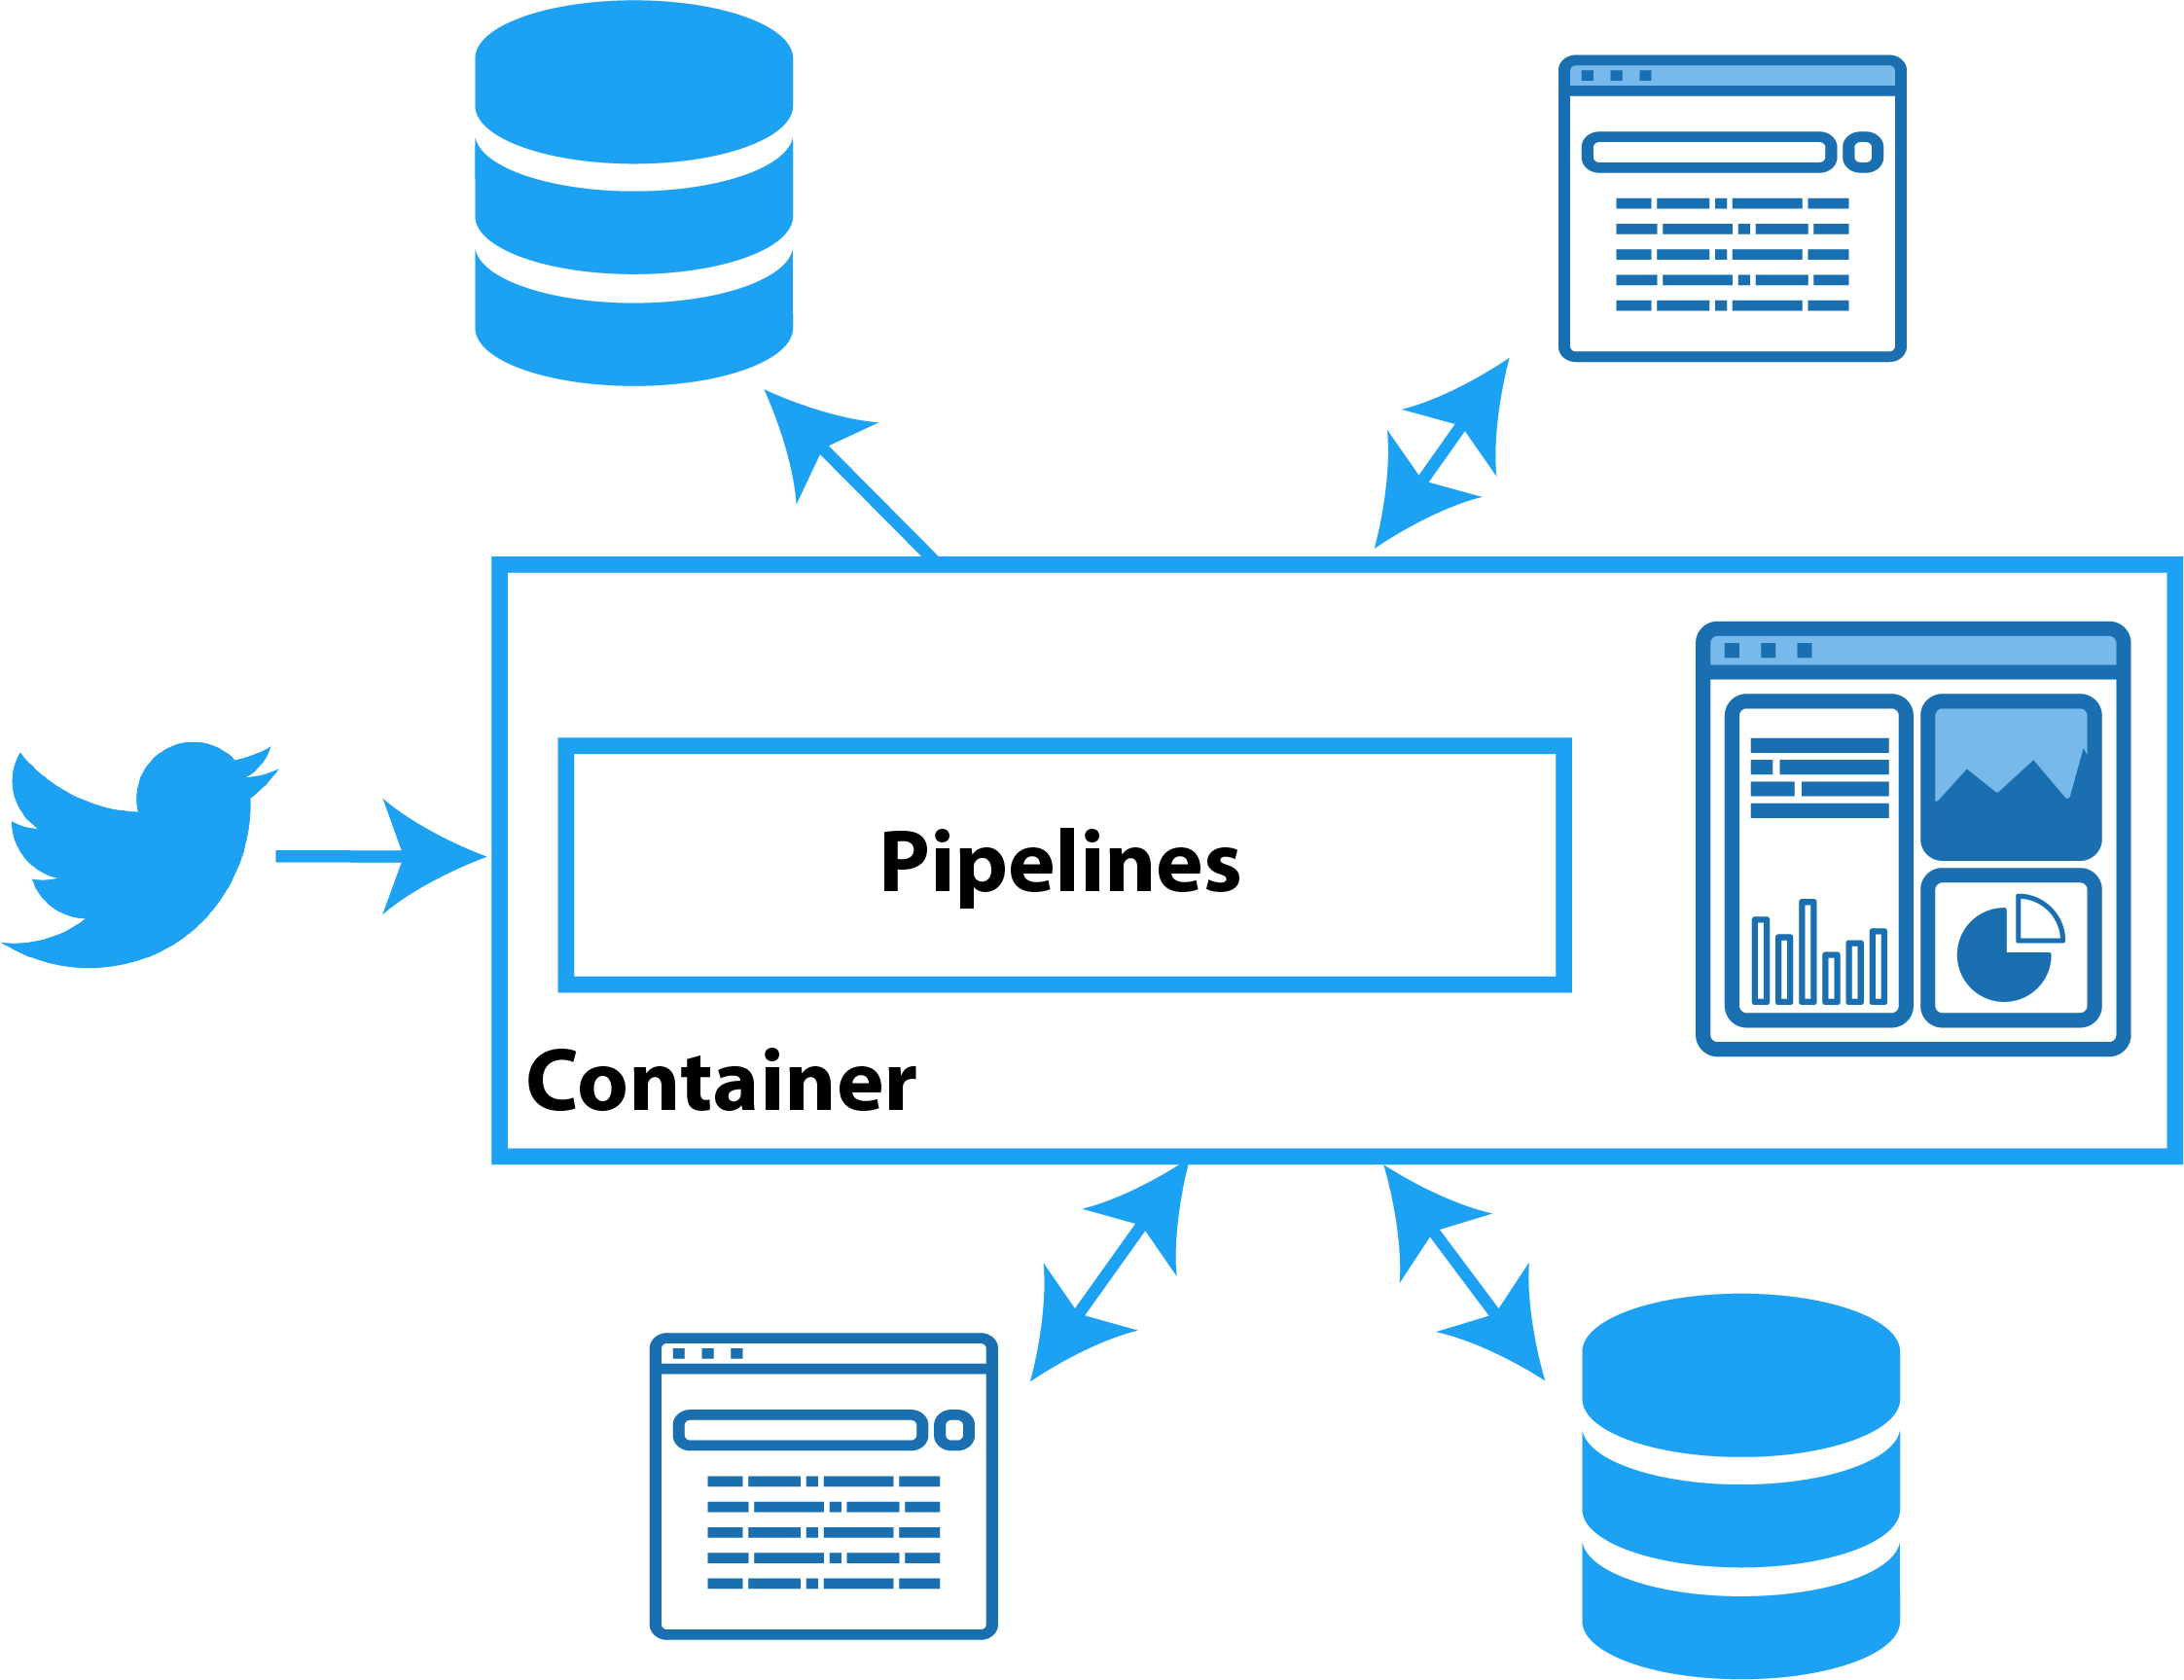
\includegraphics[scale=0.4 ]{images/architecktur_high_level_ohne.png}
	\caption{High Level L{\"o}sungsarchitekur}
	\label{fig:high_level_architecture}
\end{figure}
